% bookstyle.tex -- the designed edition of The Price of Agency ("the ledger rule").
% White pages. A single blue rule in the left column runs beside the machinery (theorems, mathematics, models);
% a double brass rule beside the receipts (code, records); a dashed grey rule beside the one fenced conjecture.
% Built by design/build_book.py from the markdown manuscript; nothing here contains manuscript text.
% Two editions from this one file. The screen edition (book.pdf) is one-sided. The print edition (book_print.pdf, built with
% `build_book.py --print`, which defines \PrintEdition) is two-sided: the text block moves away from the spine, chapters and
% parts open on right-hand pages, folios and the edge strips sit on the outer edge, and there is no cover page.
\newif\ifprinted
\ifdefined\PrintEdition\printedtrue\fi
\ifprinted\documentclass[10pt,twoside,openright]{book}\else\documentclass[10pt,oneside,openany]{book}\fi
% ---------------------------------------------------------------- page
\newlength{\ledgerw}\setlength{\ledgerw}{1.12in}      % the ledger column
\newlength{\ledgersep}\setlength{\ledgersep}{0.24in}  % gap between ledger column and text
\newlength{\outerm}\setlength{\outerm}{0.5in}
\newlength{\rightm}\setlength{\rightm}{0.72in}
\newlength{\leftm}\setlength{\leftm}{\dimexpr\outerm+\ledgerw+\ledgersep\relax}
\newlength{\ledgertotal}\setlength{\ledgertotal}{\dimexpr\ledgerw+\ledgersep\relax}
\newlength{\railoff}\setlength{\railoff}{-0.13in}
\usepackage[paperwidth=7in,paperheight=10in,left=\leftm,right=\rightm,top=0.95in,bottom=0.95in,
            headsep=0.3in,footskip=0.4in,marginparwidth=\ledgerw,marginparsep=\ledgersep]{geometry}
\newlength{\gutter}\setlength{\gutter}{0pt}
\ifprinted\setlength{\gutter}{0.11in}
  \setlength{\oddsidemargin}{\dimexpr\leftm+\gutter-1in\relax}\setlength{\evensidemargin}{\dimexpr\leftm-\gutter-1in\relax}\fi
% ---------------------------------------------------------------- type
\usepackage{amsmath,amssymb}
\usepackage[sc]{mathpazo}
\usepackage[no-math]{fontspec}
\setmainfont{TeX Gyre Pagella}[Ligatures=TeX]
\setsansfont{Fira Sans}[Scale=0.9,BoldFont={Fira Sans SemiBold},ItalicFont={Fira Sans Italic},BoldItalicFont={Fira Sans SemiBold Italic}]
\setmonofont{DejaVu Sans Mono}[Scale=0.78]
\usepackage{microtype}
\usepackage{newunicodechar}
\newunicodechar{′}{\ensuremath{'}}
\usepackage{xcolor,graphicx,tikz,enumitem,fancyhdr,array,multicol}
\usetikzlibrary{arrows.meta,calc,decorations.pathmorphing}
\usepackage[most]{tcolorbox}
\usepackage[hidelinks,pdftitle={The Price of Agency},pdfauthor={Aaron Alai}]{hyperref}
\linespread{1.06}
\setlength{\parindent}{1.15em}\setlength{\parskip}{0pt}
\frenchspacing
\clubpenalty=9000 \widowpenalty=9000 \displaywidowpenalty=9000
\setlength{\emergencystretch}{1.6em}
\relpenalty=10000 \binoppenalty=10000   % a formula in a sentence is not broken across lines
\setlist[itemize]{leftmargin=1.15em,itemsep=2pt,topsep=5pt,label={\raisebox{0.15ex}{\footnotesize\textbullet}}}
\setlist[enumerate]{leftmargin=1.5em,itemsep=2pt,topsep=5pt}
\providecommand{\tightlist}{\setlength{\itemsep}{2pt}\setlength{\parskip}{0pt}}
\setlength{\abovedisplayskip}{8pt plus 2pt minus 3pt}\setlength{\belowdisplayskip}{8pt plus 2pt minus 3pt}
% ---------------------------------------------------------------- colour
\definecolor{ink}{HTML}{1A1A1A}
\definecolor{muted}{HTML}{5B5B57}
\definecolor{hair}{HTML}{CFCEC9}
\definecolor{numeral}{HTML}{A3A29D}
\definecolor{panel}{HTML}{F4F3F0}
\definecolor{mach}{HTML}{1C5CAB}      % the machinery: harbor blue
\definecolor{rcpt}{HTML}{8A5A14}      % the receipts: ledger brass
\definecolor{fence}{HTML}{77766F}     % the fenced conjecture
\definecolor{road}{HTML}{E7E6E2}
\definecolor{car}{HTML}{8D8C88}
\definecolor{sblue}{HTML}{2A78D6}
\definecolor{sorange}{HTML}{EB6834}
\definecolor{water}{HTML}{E3ECF6}
\colorlet{trackc}{ink}
\color{ink}
% ---------------------------------------------------------------- running heads
\pagestyle{fancy}\fancyhf{}
\fancyhfoffset[L]{\ledgertotal}
\renewcommand{\headrulewidth}{0pt}
\fancyhead[L]{\sffamily\fontsize{7.5}{9}\selectfont\color{muted}The Price of Agency}
\fancyhead[R]{\sffamily\fontsize{7.5}{9}\selectfont\color{muted}\runninghead\hspace{1.4em}{\color{ink}\thepage}}
\fancypagestyle{plain}{\fancyhf{}\fancyfoot[R]{\sffamily\fontsize{7.5}{9}\selectfont\thepage}}
\ifprinted
  \fancyhf{}
  \fancyhead[LE]{\sffamily\fontsize{7.5}{9}\selectfont{\color{ink}\thepage}\hspace{1.4em}{\color{muted}The Price of Agency}}
  \fancyhead[RO]{\sffamily\fontsize{7.5}{9}\selectfont\color{muted}\runninghead\hspace{1.4em}{\color{ink}\thepage}}
  \fancypagestyle{plain}{\fancyhf{}\fancyfoot[RO,LE]{\sffamily\fontsize{7.5}{9}\selectfont\thepage}}
\fi
% where a part, a chapter or a front section opens: any page on screen, a right-hand page in print (the blank left page is bare)
\newcommand{\openpage}{\ifprinted\clearpage\ifodd\value{page}\else\thispagestyle{empty}\null\clearpage\fi\else\clearpage\fi}
\newcommand{\runninghead}{}
% ---------------------------------------------------------------- small parts
\makeatletter
\newcommand{\headfont}{\fontsize{13}{16}\selectfont\bfseries}
\newcommand{\tracknotefont}{\sffamily\fontsize{7.2}{9.4}\selectfont\color{trackc}}
% anything set in the ledger column, level with the current line (use at the start of a line)
\newcommand{\ledgerput}[1]{\llap{\smash{\parbox[t]{\ledgerw}{\raggedleft\leavevmode #1}}\hspace{\ledgersep}}}
\newif\iffirstsect\firstsectfalse
\newcommand{\tracknote}{}
% section heading: \sect{number shown in the ledger column}{title}{label}
\newcommand{\sect}[3]{\par\iffirstsect\global\firstsectfalse\else\addvspace{1.5\baselineskip}\fi\phantomsection
  \noindent\ledgerput{{\sffamily\fontsize{9}{11}\selectfont\color{trackc}#1}%
     \ifx\tracknote\@empty\else\\[5pt]{\tracknotefont\tracknote}\global\let\tracknote\@empty\fi}%
  \parbox[t]{\linewidth}{\raggedright\headfont #2}\label{#3}\par\nobreak\vspace{0.4\baselineskip}\@afterindentfalse\@afterheading}
% the book's tags
\newcommand{\stampbox}[1]{{\setlength{\fboxsep}{2.2pt}\setlength{\fboxrule}{0.5pt}\color{trackc}%
  \fbox{\upshape\sffamily\fontsize{6.2}{7}\selectfont\addfontfeature{LetterSpace=9}\bfseries #1}}}
\newcommand{\istamp}[1]{\raisebox{0.12ex}{\stampbox{#1}}}
\newcommand{\tagword}[1]{{\upshape\sffamily\fontsize{7.4}{9}\selectfont\addfontfeature{LetterSpace=7}\bfseries #1}}
% a theorem's heading: \claimhead{Theorem 5}{Activation threshold}{PROVEN}{kind}, kind 0 no tag, 1 stamp, 2 long tag
\newlength{\claimw}
\newcommand{\claimhead}[4]{\par\addvspace{1.0\baselineskip}%
   \noindent{\color{trackc}\rule{\linewidth}{0.5pt}}\par\nobreak\vspace{3pt}%
   \ifnum#4=1 \settowidth{\claimw}{\stampbox{#3}}\else\setlength{\claimw}{0pt}\fi
   \noindent\parbox[t]{\dimexpr\linewidth-\claimw-8pt}{\raggedright
      {\sffamily\bfseries\fontsize{9}{11.5}\selectfont #1}\hspace{0.7em}{\sffamily\fontsize{9}{11.5}\selectfont #2}%
      \ifnum#4=2 \par\vspace{1pt}{\sffamily\fontsize{7.4}{9.6}\selectfont\color{trackc}#3}\fi}%
   \ifnum#4=1 \hfill\stampbox{#3}\fi\par\nobreak\vspace{3.5pt}\@afterindentfalse\@afterheading}
% a run-in bold lead with a short tag
\newcommand{\axioms}[2]{\par\addvspace{1.0\baselineskip}{\centering\fontsize{13.5}{19}\selectfont
   {\sffamily\fontsize{8}{10}\selectfont\color{muted}Axiom 1}\\[1pt]#1\\[9pt]
   {\sffamily\fontsize{8}{10}\selectfont\color{muted}Axiom 2}\\[1pt]#2\par}\addvspace{1.1\baselineskip}\@afterindentfalse\@afterheading}
\newcommand{\saying}[1]{\par\addvspace{0.9\baselineskip}{\centering\itshape\fontsize{14}{19}\selectfont #1\par}\addvspace{0.9\baselineskip}\@afterindentfalse\@afterheading}
% ---------------------------------------------------------------- openers
\newcommand{\partopen}[3]{\openpage\thispagestyle{empty}\renewcommand{\runninghead}{}%
  \phantomsection\label{#3}\vspace*{1.5in}%
  \noindent\hspace*{-\ledgertotal}\parbox[t]{\dimexpr\textwidth+\ledgertotal}{\raggedright
   {\sffamily\fontsize{10}{12}\selectfont\color{muted}Part #1}\par\vspace{14pt}
   {\fontsize{34}{38}\selectfont #2}\par\vspace{0.5in}\partlist}\clearpage}
\newcommand{\partlist}{}
\newcommand{\partline}[3]{{\sffamily\fontsize{9.4}{17}\selectfont\makebox[1.6em][l]{\color{muted}#1}#2\hspace{0.8em}{\color{muted}\pageref{#3}}\par}}
\newcommand{\chapteropen}[4]{\openpage\thispagestyle{plain}\renewcommand{\runninghead}{#3}\phantomsection\label{#4}%
  \noindent\hspace*{-\ledgertotal}{\sffamily\fontsize{8.5}{10}\selectfont\color{muted}#1}\par\vspace{0.62in}%
  \noindent\llap{\smash{\fontsize{66}{66}\selectfont\color{numeral}#2}\hspace{\ledgersep}}%
  \parbox[t]{\linewidth}{\raggedright\fontsize{31}{35}\selectfont #3}\par\vspace{0.3in}\@afterindentfalse\@afterheading}
\newcommand{\plainsect}[2]{\par\addvspace{1.6\baselineskip}\phantomsection\noindent\parbox[t]{\linewidth}{\raggedright\fontsize{15}{18.5}\selectfont\bfseries #1}\label{#2}%
  \par\nobreak\vspace{0.5\baselineskip}\@afterindentfalse\@afterheading}
% route map under a chapter title
\newlength{\mapcell}\setlength{\mapcell}{\dimexpr(\textwidth+\ledgertotal)/6\relax}
\newcommand{\mapbar}[1]{%
  \ifnum#1=0 {\color{ink}\rule{\dimexpr\mapcell-6pt}{2.6pt}}\fi
  \ifnum#1=1 {\color{mach}\rule{\dimexpr\mapcell-6pt}{2.6pt}}\fi
  \ifnum#1=2 {\color{rcpt}\rlap{\smash{\rule[1.7pt]{\dimexpr\mapcell-6pt}{0.9pt}}}\rule{\dimexpr\mapcell-6pt}{0.9pt}\rule{0pt}{2.6pt}}\fi
  \ifnum#1=3 {\color{fence}\rlap{\smash{\tikz[baseline=0pt]{\draw[fence,line width=1.4pt,dash pattern=on 3.2pt off 2.2pt] (0,0.6pt) -- (\dimexpr\mapcell-6pt,0.6pt);}}}\rule{0pt}{2.6pt}\hspace{\dimexpr\mapcell-6pt}}\fi}
\newcommand{\mapcellbox}[4]{\parbox[t]{\mapcell}{\raggedright\leavevmode\mapbar{#1}\\[3pt]%
  {\bfseries\fontsize{7.6}{9.5}\selectfont #2}\\{\fontsize{8.4}{10.4}\selectfont #3}\\%
  {\color{muted}\fontsize{7.6}{9.5}\selectfont page \pageref{#4}}}}
\newcommand{\routemap}[1]{\noindent\hspace*{-\ledgertotal}\parbox[t]{\dimexpr\textwidth+\ledgertotal+2pt}{\sffamily\raggedright #1}\par\vspace{0.22in}}
\newcommand{\maprowbreak}{\par\vspace{10pt}}
\makeatother
% ---------------------------------------------------------------- the kinds of text
\tcbset{trackbase/.style={enhanced,breakable,parbox=false,boxrule=0pt,frame hidden,arc=0pt,outer arc=0pt,
  boxsep=0pt,left=0pt,right=0pt,top=0pt,bottom=0pt,before skip=1.5\baselineskip,after skip=0pt,
  pad at break=0pt,colupper=ink,interior hidden}}
\ifprinted
  \tcbset{trackbase/.append style={check odd page=true}}
  \newcommand{\edgestrip}[1]{\tcbifoddpage{\fill[#1] ([xshift=\rightm-\gutter-6.5pt]frame.north east) rectangle ([xshift=\rightm-\gutter]frame.south east);}%
     {\fill[#1] ([xshift=-\leftm+\gutter]frame.north west) rectangle ([xshift=-\leftm+\gutter+6.5pt]frame.south west);}}
\else
  \newcommand{\edgestrip}[1]{\fill[#1] ([xshift=\rightm-6.5pt]frame.north east) rectangle ([xshift=\rightm]frame.south east);}
\fi
\newcommand{\contlabel}[2]{\node[anchor=north east,inner sep=0pt,font=\sffamily\fontsize{7.2}{9}\selectfont,text=#1]
   at ([xshift=-\ledgersep,yshift=-1pt]frame.north west) {#2, continued};}
\newtcolorbox{machbox}[1][]{trackbase,#1,borderline west={1.7pt}{\railoff}{mach},
  overlay={\edgestrip{mach}},overlay middle and last={\edgestrip{mach}\contlabel{mach}{the machinery}}}
\newtcolorbox{rcptbox}[1][]{trackbase,#1,borderline west={0.8pt}{\railoff}{rcpt},borderline west={0.8pt}{\dimexpr\railoff-2.2pt}{rcpt},
  overlay={\edgestrip{rcpt}},overlay middle and last={\edgestrip{rcpt}\contlabel{rcpt}{the receipts}}}
\newtcolorbox{fencebox}[1][]{trackbase,#1,borderline west={1.3pt}{\railoff}{fence,dash pattern=on 4pt off 3pt},
  overlay middle and last={\contlabel{fence}{fenced}}}
% a boxed passage (the manuscript's block quotes); the argument is the rail style of the track it sits in
\tcbset{panelbase/.style={enhanced,breakable,parbox=false,boxrule=0.4pt,colframe=hair,colback=panel,arc=1.5pt,
  left=9pt,right=9pt,top=7pt,bottom=7pt,boxsep=0pt,before skip=1.0\baselineskip,after skip=1.0\baselineskip,colupper=ink,
  fontupper=\fontsize{9.4}{13.4}\selectfont}}
\newtcolorbox{panelplain}{panelbase}
\newtcolorbox{panelmach}{panelbase,borderline west={1.7pt}{\railoff}{mach},overlay={\edgestrip{mach}}}
\newtcolorbox{panelrcpt}{panelbase,borderline west={0.8pt}{\railoff}{rcpt},borderline west={0.8pt}{\dimexpr\railoff-2.2pt}{rcpt},overlay={\edgestrip{rcpt}}}
\newtcolorbox{panelfence}{panelbase,borderline west={1.3pt}{\railoff}{fence,dash pattern=on 4pt off 3pt}}
% track environments: the argument is the note printed in the ledger column where the track begins (may be empty)
\newenvironment{machinery}[2][]{\par\colorlet{trackc}{mach}\gdef\tracknote{#2}\global\firstsecttrue\begin{machbox}[#1]}{\end{machbox}\par}
\newenvironment{receipts}[2][]{\par\colorlet{trackc}{rcpt}\gdef\tracknote{#2}\global\firstsecttrue\begin{rcptbox}[#1]}{\end{rcptbox}\par}
\newenvironment{fenced}[2][]{\par\colorlet{trackc}{fence}\gdef\tracknote{#2}\global\firstsecttrue\begin{fencebox}[#1]}{\end{fencebox}\par}
% one ruled paragraph outside the numbered sections (Chapter 2); its margin note is set by the builder at the paragraph's first word
\newenvironment{ruled}{\par\colorlet{trackc}{mach}\begin{machbox}[before skip=0.9\baselineskip,after skip=0.9\baselineskip]}{\end{machbox}\par}
\newcommand{\rulednote}[1]{\noindent\ledgerput{{\tracknotefont #1}}}
\newenvironment{everyone}{\par\colorlet{trackc}{ink}\gdef\tracknote{}}{\par}
% ---------------------------------------------------------------- pictures
\newcommand{\figcap}[2]{\par\vspace{5pt}\noindent{\sffamily\fontsize{8}{10.6}\selectfont\color{ink}\textbf{Figure #1}\hspace{0.6em}#2\par}}
\newcommand{\bookfigure}[3]{\par\addvspace{1.0\baselineskip}\noindent\begin{minipage}{\linewidth}\noindent\includegraphics[width=\linewidth]{#1}\figcap{#2}{#3}\end{minipage}\par\addvspace{1.0\baselineskip}}
% on story pages a picture that does not fit where it is called moves to the top of the next page and the text runs on
\renewcommand{\topfraction}{0.92}\renewcommand{\bottomfraction}{0.6}\renewcommand{\textfraction}{0.06}\renewcommand{\floatpagefraction}{0.85}
\setlength{\intextsep}{1.0\baselineskip}\setlength{\textfloatsep}{1.3\baselineskip}
\newcommand{\bookfigurefloat}[3]{\begin{figure}[!ht]\noindent\includegraphics[width=\linewidth]{#1}\figcap{#2}{#3}\end{figure}}
\newcommand{\bookfigurewidefloat}[3]{\begin{figure}[!ht]\noindent\hspace*{-\ledgertotal}\includegraphics[width=\dimexpr\linewidth+\ledgertotal]{#1}\figcap{#2}{#3}\end{figure}}
\newcommand{\booktikzfloat}[3]{\begin{figure}[!ht]\noindent\input{#1}\figcap{#2}{#3}\end{figure}}
% tables (the builder sets each pipe table of the manuscript with these)
% break here only if less than #1 is left on the page. These pages have no stretch of their own, so TeX rates every break on
% them as equally bad and keeps the last one; a break offered with stretch s is preferred only while the room left is under
% 4.64 s (badness below 10000). Hence the stretch is #1/4.65, and the penalty is zero.
\newcommand{\tableneed}[1]{\par\vskip 0pt plus \dimexpr #1*215/1000\relax\penalty 0\vskip 0pt plus -\dimexpr #1*215/1000\relax\relax}
\newcommand{\tablefont}{\sffamily\fontsize{7.5}{9.9}\selectfont}
\newcommand{\tablerule}{\par\nobreak\vskip 1.6pt{\color{muted}\hrule height 0.45pt}\vskip 2.4pt}
\newcommand{\tablehair}{\par\nobreak\vskip 1.4pt{\color{hair}\hrule height 0.3pt}\vskip 2.2pt}
\newcommand{\tablerow}[1]{\par\noindent #1}
\makeatletter
\newenvironment{booktable}{\par\addvspace{0.75\baselineskip}\begingroup\tablefont\setlength{\parindent}{0pt}\setlength{\parskip}{0pt}%
  {\color{muted}\hrule height 0.45pt}\nobreak\vskip 2.4pt}
  {\par\endgroup\addvspace{0.85\baselineskip}\@afterindentfalse\@afterheading}
\makeatother
% a picture that also takes the ledger column (story pages only: nothing else lives in that column there)
\newcommand{\bookfigurewide}[3]{\par\addvspace{1.0\baselineskip}\noindent\begin{minipage}{\linewidth}\noindent\hspace*{-\ledgertotal}\includegraphics[width=\dimexpr\linewidth+\ledgertotal]{#1}\figcap{#2}{#3}\end{minipage}\par\addvspace{1.0\baselineskip}}
\newcommand{\booktikz}[3]{\par\addvspace{1.0\baselineskip}\noindent\begin{minipage}{\linewidth}\noindent\input{#1}\figcap{#2}{#3}\end{minipage}\par\addvspace{1.0\baselineskip}}
% ---------------------------------------------------------------- the cover (design/fig/cover_art.pdf is drawn by make_figures.py)
\newcommand{\coverpage}{\noindent\begin{tikzpicture}[remember picture,overlay]
  \node[anchor=south,inner sep=0pt] at ([xshift=0.45in,yshift=1.7in]current page.south) {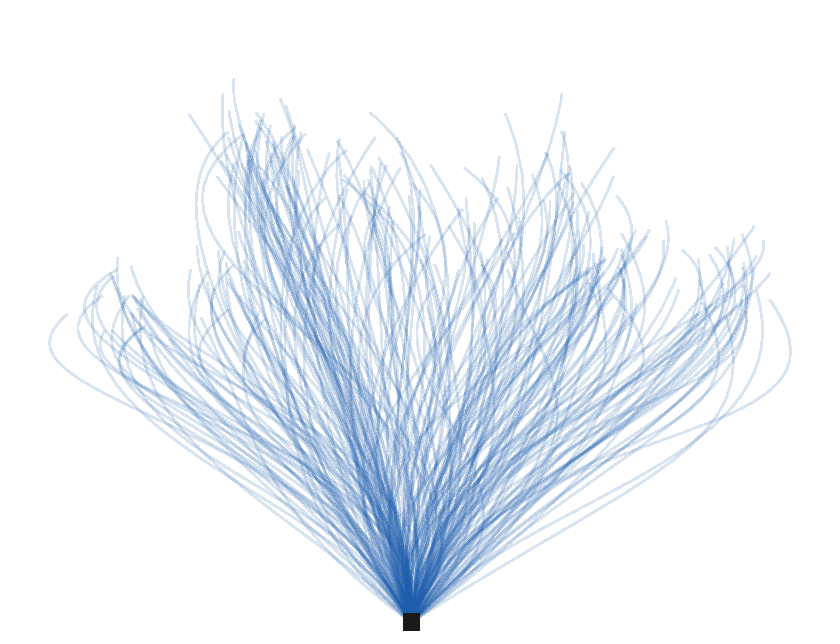
\includegraphics[width=5.6in]{fig/cover_art}};
  \fill[mach] ([xshift=0.62in]current page.north west) rectangle ([xshift=0.62in+2.4pt]current page.south west);
  \fill[rcpt] ([xshift=0.62in+7pt]current page.north west) rectangle ([xshift=0.62in+8.1pt]current page.south west);
  \fill[rcpt] ([xshift=0.62in+10.3pt]current page.north west) rectangle ([xshift=0.62in+11.4pt]current page.south west);
  \node[anchor=north west,inner sep=0pt,align=left,text=ink] at ([xshift=1.12in,yshift=-1.25in]current page.north west) {\fontsize{50}{54}\selectfont The Price\\[5pt]\fontsize{50}{54}\selectfont of Agency};
  \node[anchor=north west,inner sep=0pt,align=left,text=ink] at ([xshift=1.12in,yshift=-3.05in]current page.north west) {\fontsize{14}{20}\selectfont\itshape Freedom, measured. Theft, priced.\\\fontsize{14}{20}\selectfont\itshape No opinions required.};
  \node[anchor=south west,inner sep=0pt,align=left,text=ink] at ([xshift=1.12in,yshift=0.78in]current page.south west) {\sffamily\fontsize{12}{15}\selectfont Aaron Alai\\[2pt]\sffamily\fontsize{8.6}{12}\selectfont\color{muted}with Claude (Anthropic) as mathematical collaborator};
\end{tikzpicture}}
% ---------------------------------------------------------------- the index (its entries are written by design/make_index.py)
\newcommand{\indexopen}{\openpage\thispagestyle{plain}\renewcommand{\runninghead}{Index}\phantomsection\label{index}%
  \noindent\hspace*{-\ledgertotal}\parbox[t]{\dimexpr\textwidth+\ledgertotal}{\raggedright\fontsize{31}{35}\selectfont Index}\par\vspace{0.22in}%
  \noindent{\sffamily\fontsize{7.6}{10.4}\selectfont\color{muted}Words the book uses on nearly every page are listed at the passages that define them or turn on them. The theorems follow, by number.\par}\vspace{0.16in}%
  \begin{multicols}{2}\sffamily\fontsize{7.6}{10.6}\selectfont\raggedright\setlength{\parskip}{1.2pt}\setlength{\parindent}{0pt}}
\newcommand{\indexentry}[2]{\par\hangindent=1.1em\hangafter=1\noindent #1\enspace{\color{muted}#2}}
\newcommand{\indexclaims}{\par\vspace{1.0\baselineskip}\noindent{\bfseries Theorems and results, where stated}\par\vspace{0.3\baselineskip}}
\newcommand{\indexclose}{\end{multicols}}
% ---------------------------------------------------------------- key to the pages
\newcommand{\swatch}[1]{\tikz[baseline=-0.6ex]{#1}}
\newcommand{\keyrow}[3]{\noindent\makebox[0.42in][l]{#1}\parbox[t]{\dimexpr\linewidth-0.42in}{\raggedright\sffamily\fontsize{8.6}{12}\selectfont\textbf{#2}\hspace{0.6em}#3}\par\vspace{6pt}}
\newcommand{\pagekey}{\par\addvspace{0.9\baselineskip}\noindent\begin{minipage}{\linewidth}
 {\color{hair}\rule{\linewidth}{0.5pt}}\par\vspace{7pt}
 \keyrow{\swatch{\draw[hair,line width=0.5pt,fill=white] (0,-0.13) rectangle (0.26in,0.13);}}{No rule}{§1 and §2: the idea and the story. For every reader.}
 \keyrow{\swatch{\draw[mach,line width=1.7pt] (0.13in,-0.16) -- (0.13in,0.16);}}{Single blue rule}{§3 onward: theorems, mathematics, models. The machinery.}
 \keyrow{\swatch{\draw[rcpt,line width=0.8pt] (0.12in,-0.16) -- (0.12in,0.16);\draw[rcpt,line width=0.8pt] (0.12in+2.2pt,-0.16) -- (0.12in+2.2pt,0.16);}}{Double brass rule}{§6 and the public record: code, files, data. The receipts.}
 \keyrow{\swatch{\draw[fence,line width=1.3pt,dash pattern=on 4pt off 3pt] (0.13in,-0.16) -- (0.13in,0.16);}}{Dashed rule}{Chapter 12 only: a conjecture, fenced.}
 \vspace{-1pt}{\color{hair}\rule{\linewidth}{0.5pt}}\end{minipage}\par\addvspace{0.9\baselineskip}}
% ---------------------------------------------------------------- contents
\newcommand{\tocpart}[3]{\par\addvspace{13pt}\noindent\hspace*{-\ledgertotal}\makebox[\ledgertotal][l]{\sffamily\fontsize{8.4}{11}\selectfont\color{muted}Part #1}%
  {\sffamily\bfseries\fontsize{10}{13}\selectfont #2}\par\vspace{3pt}}
\newcommand{\tocchap}[3]{\noindent\makebox[1.7em][l]{\sffamily\fontsize{9}{15}\selectfont\color{muted}#1}{\fontsize{10.3}{15.5}\selectfont #2}%
  {\color{hair}\,\leaders\hbox to 0.5em{\hss.\hss}\hfill\,}{\sffamily\fontsize{9}{15}\selectfont\pageref{#3}}\par}
\newcommand{\tocessay}[2]{\noindent\makebox[1.7em][l]{}{\fontsize{10.3}{15.5}\selectfont\itshape #1}{\color{hair}\,\leaders\hbox to 0.5em{\hss.\hss}\hfill\,}{\sffamily\fontsize{9}{15}\selectfont\pageref{#2}}\par}
\newcommand{\tocfront}[2]{\noindent{\fontsize{10.3}{15.5}\selectfont #1}{\color{hair}\,\leaders\hbox to 0.5em{\hss.\hss}\hfill\,}{\sffamily\fontsize{9}{15}\selectfont\pageref{#2}}\par}
\newcommand{\frontsect}[2]{\openpage\thispagestyle{plain}\renewcommand{\runninghead}{#1}\phantomsection\label{#2}%
  \vspace*{0.35in}\noindent\parbox[t]{\linewidth}{\raggedright\fontsize{24}{28}\selectfont #1}\par\vspace{0.3in}}
% ---------------------------------------------------------------- displayed mathematics
\makeatletter
\newenvironment{dispmath}{\par\addvspace{9pt}\begingroup\centering$\displaystyle}{$\par\endgroup\addvspace{9pt}\@afterindentfalse\@afterheading}
\makeatother
